../cictikz/src/cictikz/data/tex/cictikz_preamble.tex

% Intrinsic gain against gate voltage.
%
% The quantity plotted is gm/gds, the most gain a single transistor can
% give however it is loaded. It falls by more than half across the sweep,
% from about 13 near threshold to 5 in strong inversion, and the fall is
% monotonic.
%
% That is the trade the chapter keeps returning to. Driving a device hard
% buys speed and headroom and costs gain, and no amount of circuit
% cleverness recovers what the device itself does not have.
%
% Generated by py/tikzplot.py. Edit the script in ex/ that
% produced it and re-run that, not this file.

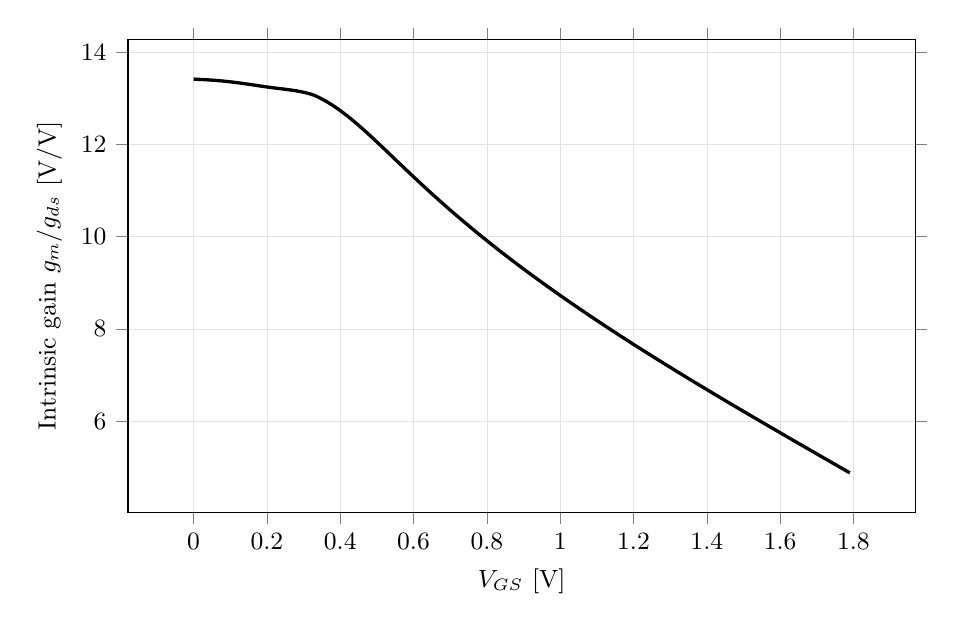
\begin{tikzpicture}[thick]

\begin{axis}[
  width=10.0cm,
  height=6.0cm,
  scale only axis,
  grid=both,
  grid style={gray!22, very thin},
  tick align=outside,
  tick label style={font=\small},
  label style={font=\small},
  title style={font=\small, yshift=-1mm},
  legend cell align=left,
  legend style={font=\small, draw=gray!50, fill=white, fill opacity=0.85, text opacity=1},
  xlabel={$V_{GS}$ [V]},
  ylabel={Intrinsic gain $g_m/g_{ds}$ [V/V]}
]
\addplot[black, very thick, mark=none] coordinates {(0,13.419) (0.01,13.415) (0.02,13.412) (0.03,13.407) (0.04,13.403) (0.05,13.397) (0.06,13.391) (0.07,13.385) (0.08,13.377) (0.09,13.369) (0.1,13.361) (0.11,13.351) (0.12,13.341) (0.13,13.33) (0.14,13.319) (0.15,13.308) (0.16,13.296) (0.17,13.284) (0.18,13.272) (0.19,13.261) (0.2,13.249) (0.21,13.239) (0.22,13.228) (0.23,13.218) (0.24,13.209) (0.25,13.199) (0.26,13.188) (0.27,13.177) (0.28,13.165) (0.29,13.15) (0.3,13.134) (0.31,13.115) (0.32,13.093) (0.33,13.066) (0.34,13.029) (0.35,12.988) (0.36,12.944) (0.37,12.897) (0.38,12.847) (0.39,12.793) (0.4,12.737) (0.41,12.677) (0.42,12.616) (0.43,12.551) (0.44,12.485) (0.45,12.417) (0.46,12.347) (0.47,12.276) (0.48,12.203) (0.49,12.13) (0.5,12.055) (0.51,11.98) (0.52,11.905) (0.53,11.829) (0.54,11.753) (0.55,11.677) (0.56,11.601) (0.57,11.525) (0.58,11.449) (0.59,11.374) (0.6,11.299) (0.61,11.225) (0.62,11.15) (0.63,11.077) (0.64,11.004) (0.65,10.931) (0.66,10.86) (0.67,10.788) (0.68,10.718) (0.69,10.647) (0.7,10.578) (0.71,10.509) (0.72,10.441) (0.73,10.373) (0.74,10.306) (0.75,10.239) (0.76,10.173) (0.77,10.107) (0.78,10.042) (0.79,9.9777) (0.8,9.9137) (0.81,9.8502) (0.82,9.7872) (0.83,9.7247) (0.84,9.6627) (0.85,9.6011) (0.86,9.5399) (0.87,9.4792) (0.88,9.4189) (0.89,9.3591) (0.9,9.2996) (0.91,9.2405) (0.92,9.1818) (0.93,9.1235) (0.94,9.0656) (0.95,9.008) (0.96,8.9508) (0.97,8.8939) (0.98,8.8373) (0.99,8.7811) (1,8.7252) (1.01,8.6696) (1.02,8.6143) (1.03,8.5593) (1.04,8.5046) (1.05,8.4502) (1.06,8.396) (1.07,8.3422) (1.08,8.2885) (1.09,8.2352) (1.1,8.1821) (1.11,8.1293) (1.12,8.0766) (1.13,8.0243) (1.14,7.9721) (1.15,7.9202) (1.16,7.8685) (1.17,7.8171) (1.18,7.7658) (1.19,7.7147) (1.2,7.6639) (1.21,7.6132) (1.22,7.5627) (1.23,7.5124) (1.24,7.4623) (1.25,7.4124) (1.26,7.3626) (1.27,7.313) (1.28,7.2636) (1.29,7.2143) (1.3,7.1652) (1.31,7.1163) (1.32,7.0675) (1.33,7.0188) (1.34,6.9703) (1.35,6.9219) (1.36,6.8736) (1.37,6.8255) (1.38,6.7775) (1.39,6.7296) (1.4,6.6818) (1.41,6.6341) (1.42,6.5866) (1.43,6.5391) (1.44,6.4918) (1.45,6.4445) (1.46,6.3974) (1.47,6.3503) (1.48,6.3034) (1.49,6.2565) (1.5,6.2097) (1.51,6.1629) (1.52,6.1163) (1.53,6.0697) (1.54,6.0232) (1.55,5.9768) (1.56,5.9304) (1.57,5.8841) (1.58,5.8378) (1.59,5.7916) (1.6,5.7454) (1.61,5.6993) (1.62,5.6533) (1.63,5.6072) (1.64,5.5613) (1.65,5.5153) (1.66,5.4694) (1.67,5.4235) (1.68,5.3777) (1.69,5.3319) (1.7,5.2861) (1.71,5.2403) (1.72,5.1946) (1.73,5.1488) (1.74,5.1031) (1.75,5.0574) (1.76,5.0117) (1.77,4.9661) (1.78,4.9204) (1.79,4.8747)};
\end{axis}

\end{tikzpicture}
\end{document}
